\documentclass[output=paper]{langscibook}
\author{Masahiko Takahashi\affiliation{Yamagata University}\orcid{}}
\title{Some notes on the scope properties of nominative objects in Japanese}
\abstract{This chapter aims to provide novel support for a phrasal complementation approach to restructuring phenomena on the basis of an analysis of some novel observations concerning the scope properties of nominative objects in Japanese. It is first shown that nominative objects must take scope under the potential suffix when subjects receive an instrumental case. It is then argued that the obligatory narrow scope of nominative objects under consideration follows from the phrasal complementation approach, which dictates that the nominative object is base-generated below the potential suffix. The observation is difficult to capture with an alternative complex head approach, in which the nominative object is always base-generated above the potential suffix.}

\begin{document}
\SetupAffiliations{mark style=none}
\maketitle

\section{Introduction}
Although there have been several proposals on restructuring (clause union) constructions (see \citealt{Miyagawa1987}; \citealt{SaitoHoshi1998}; \citealt{Cinque2006}; \citealt{wurmbrand2001, Wurmbrand2015a,Wurmbrand2015b}; \citealt{bobaljikwurmbrand2005, bobaljikwurmbrand2007}; \citealt{nomura2005}; \citealt{takahashi2011}; \citealt{shimamurawurmbrand2014} among others), the precise nature of restructuring is still under debate. This chapter aims to provide novel support for the phrasal complementation approach advocated by \citeauthor{wurmbrand2001} (\citeyear{wurmbrand2001},
\citeyear{Wurmbrand2015a}, \citeyear{Wurmbrand2015b}), \citet{bobaljikwurmbrand2005, bobaljikwurmbrand2007}, \citet{nomura2005}, \citet{takahashi2011}, and \citet{shimamurawurmbrand2014}, among others, on the basis of an analysis of novel observations concerning the scope properties of nominative objects in Japanese.

It has been observed in the literature that while transitive objects in Japanese usually must receive the accusative case, they can receive the nominative case when a transitive predicate is accompanied by a potential suffix \citep{kuno1973}:

\ea \label{takaha1}
\gll {Kodomo-tati-ga} {kanzirensyuu-o/*ga} {tuzuke-ru.}\\
	child-\textsc{pl}-\textsc{nom}       kanji.practice-\textsc{acc/nom} continue-\textsc{prs}\\
\glt `Children continue kanji practice.’
\z

\ea \label{takaha2}
\gll {Kodomo-tati-ga} {kanzirensyuu-o/ga} {tuzuke-rare-ru.}\\
	child-\textsc{pl}-\textsc{nom}       kanji.practice-\textsc{acc/nom} continue-can-\textsc{prs}\\
\glt `Children can continue kanji practice.’
\z

The transitive verb \emph{tuzuke} ‘continue’ in (\ref{takaha1}) can only assign the accusative case to the object \emph{kanzirensyuu} ‘kanji practice.’ In addition, when \emph{tuzuke} ‘continue’ is accompanied by the potential suffix \emph{-rare} ‘can’, as in (\ref{takaha2}), the object \emph{kanzirensyuu} ‘kanji practice’ can receive either the accusative case or the nominative case. Notably, accusative and nominative objects behave differently with respect to scope (see \citealt{Sano1985}; \citealt{Tada1992}; \citealt{Koizumi1998,Koizumi2008}; \citealt{Ura1999}; \citealt{Yatsushiro1999}; \citealt{Takano2003}; \citealt{nomura2005}; \citealt{bobaljikwurmbrand2007}; \citealt{takahashi2011}; \citealt{shimamurawurmbrand2014}; \citealt{FunakoshiTakahashi2014}; \citealt{ochisaruwatari2014a}; \citealt{kasai2018} among others). 

\begin{exe}
\ex 

\begin{xlist}

\ex \label{takaha3a}
\gll {Kodomo-tati-ga} {kanzirensyuu-dake-o} {tuzuke-rare-ru.}\\
	child-\textsc{pl}-\textsc{nom}       kanji.practice-only-\textsc{acc} continue-can-\textsc{prs}\\
\glt ‘Children can continue only kanji practice.’\\
	‘Children can continue kanji practice without doing any other things.’ (can \textgreater{} only)\\
 	`It is only kanji practice that children can continue.’\\
(?*only \textgreater{} can)
\\

\ex \label{takaha3b}
\gll {Kodomo-tati-ga} {kanzirensyuu-dake-ga} {tuzuke-rare-ru.}\\
	child-\textsc{pl}-\textsc{nom}       kanji.practice-only-\textsc{nom} continue-can-\textsc{prs}\\
\glt `Children can continue only kanji practice.’\\
`Children can continue kanji practice without doing any other things.' (can \textgreater{} only)\\
`It is only kanji practice that children can continue.’ (only \textgreater{} can)

\end{xlist}
\end{exe}

The verb \emph{tuzuke} ‘continue’ in (\ref{takaha3a}) and (\ref{takaha3b}) is accompanied by the potential suffix \emph{-rare} ‘can’, and the two examples differ only in the case of the object. Interestingly, while the accusative object in (\ref{takaha3a}) must take scope under the potential suffix, the nominative object in (\ref{takaha3b}) can take scope over the potential suffix.\footnote{Contrary to earlier works that assume that nominative objects must take scope over the potential suffix (see \citealt{Tada1992}; \citealt{Koizumi1998}; \citealt{SaitoHoshi1998}; \citealt{Takano2003}), I assume, in alignment with more recent works, that nominative objects can take scope under the potential suffix (see \citealt{nomura2005}; \citealt{Koizumi2008}; \citealt{takahashi2011}; \citealt{FunakoshiTakahashi2014}; \citealt{ochisaruwatari2014a}; \citealt{kasai2018}). See below for discussion.} The rest of this chapter elucidates that the scope properties of nominative objects interact with the case of subjects. It is then argued that the observation under consideration provides further credence to the phrasal complementation approach, which dictates that the nominative object is base-generated below the potential suffix (see \citealt{wurmbrand2001}; \citealt{bobaljikwurmbrand2005,bobaljikwurmbrand2007}; \citealt{nomura2005}; \citealt{Takano2011}; \citealt{FunakoshiTakahashi2014}; \citealt{shimamurawurmbrand2014}). Conversely, the observation is hard to capture with an alternative complex head approach (\citealt{SaitoHoshi1998}), in which the nominative object is always base-generated above the potential suffix.

This chapter is organized as follows. Section \ref{takahas2} shows that nominative objects must take scope under the potential suffix when a co-occurring subject receives an instrumental case. Section \ref{takahas3} provides an analysis of the data provided in Section \ref{takahas2}, essentially following \citet{Kishimoto2010} and \citet{shimamurawurmbrand2014}. Section \ref{takahas4} discusses an alternative analysis in terms of the complex head approach and shows that such an analysis has difficulty capturing the data in question. Section \ref{takahas5} presents further consequences of the proposed analysis, and Section \ref{takahas6} concludes this chapter.

\section{Instrumental subjects and the scope properties of nominative objects} \label{takahas2}

This section provides the core observations discussed in this chapter. In particular, it is shown that nominative objects must take scope under the potential suffix when co-occurring subjects receive an instrumental case. While the above examples all involve nominative subjects, it is well known that Japanese allows several non-nominative subjects (see \citealt{kishimoto2017case} for an overview). Below is an example of a subject that receives the instrumental case (see \citealt{Kishimoto2005,Kishimoto2010}; \citealt{Takubo1984}; \citealt{Inoue1998}):


\begin{exe}
\ex 
\begin{xlist}

\ex \label{takaha4a}
\gll {Kodomo-tati-ga} {kanzirensyuu-o} {tuzuke-ru.}\\
	child-\textsc{pl}-\textsc{nom}  kanji.practice-\textsc{acc} continue-\textsc{prs} (cf. (\ref{takaha1}))\\ 
	
\ex \label{takaha4b}
\gll {Kodomo-tati-de} {kanzirensyuu-o} {tuzuke-ru.}\\
	child-\textsc{pl}-with       kanji.practice-\textsc{acc} continue-\textsc{prs}\\
\glt `Children continue kanji practice.' \\
\end{xlist}


\end{exe}

While the subject in (\ref{takaha4a}) receives the nominative marker \emph{-ga}, the subject in (\ref{takaha4b}) receives \emph{-de}, which is usually employed to mark instruments (e.g., \emph{naifu-de} `with a knife’). Following \citet{Kishimoto2005,Kishimoto2010}, I dub subjects that receive \emph{-de instrumental subjects}.\footnote{Instrumental subjects must be plural (see \citealt{Takubo1984, Kishimoto2005, Kishimoto2010}). I thus use plural subjects for all the relevant examples in the text.} As shown below, instrumental subjects can appear in the potential construction.

\begin{exe}
\ex \label{takaha5}
\begin{xlist}
\ex \label{takaha5a}
\gll {Kodomo-tati-ga} {kanzirensyuu-o/ga} {tuzuke-rare-ru.}\\
	child-\textsc{pl}-\textsc{nom}  kanji.practice-\textsc{acc/nom} continue-can-\textsc{prs} (= (\ref{takaha2}))\\ 
	
\ex \label{takaha5b}
\gll {Kodomo-tati-de} {kanzirensyuu-o/ga} {tuzuke-rare-ru.}\\
	child-\textsc{pl}-with       kanji.practice-\textsc{acc/nom} continue-can-\textsc{prs}\\
\glt `Children can continue kanji practice.' \\
\end{xlist}
\end{exe}

The transitive verb \emph{tuzuke} ‘continue’ is accompanied by the potential suffix \emph{-rare} ‘can’, and the object can receive either the accusative or nominative case. The subject of this construction can receive either the nominative case, as in (\ref{takaha5a}), or the instrumental case, as in (\ref{takaha5b}). Significantly, the scope of nominative objects appears to correlate with the case of the subjects (see \citealt{Ebina2020}):

\begin{exe}
\ex 
\begin{xlist}
\ex \label{takaha6a}
\gll {Kodomo-tati-ga} {kanzirensyuu-dake-ga} {tuzuke-rare-ru.}\\
	child-\textsc{pl}-\textsc{nom}       kanji.practice-only-\textsc{nom} continue-can-\textsc{prs}\\
\glt `Children can continue only kanji practice.’ (= (\ref{takaha3b}))\\
‘Children can continue kanji practice without doing other things.’ (can \textgreater{} only)\\
‘It is only kanji practice that children can continue.’ (only \textgreater{} can)
\\

\ex \label{takaha6b}
\gll {Kodomo-tati-de} {kanzirensyuu-dake-ga} {tuzuke-rare-ru.}\\
	child-\textsc{pl}-with kanji.practice-only-\textsc{nom} continue-can-\textsc{prs}\\
\glt `Children can continue only kanji practice.’\\
`Children can continue kanji practice without doing any other things.' (can \textgreater{} only)\\
`It is only kanji practice that children can continue.’ (?*only \textgreater{} can)
\end{xlist}
\end{exe}

As reported in the literature, the nominative object can take scope over the potential suffix when the former appears with the nominative subject, as in (\ref{takaha6a}). However, the nominative object must take scope under the potential suffix when the former appears with the instrumental subject, as in (\ref{takaha6b}). The following section provides an analysis of the contrast between (\ref{takaha6a}) and (\ref{takaha6b}), essentially following the analysis of the instrumental subjects proposed by \citet{Kishimoto2010} and the structure of the potential construction proposed by \citet{shimamurawurmbrand2014}.

\section{An analysis}\label{takahas3}

\subsection{Instrumental subjects}
\citet{Kishimoto2010} makes two important claims about nominative and instrumental subjects, each of which is addressed below:

\begin{exe}
\ex 
\begin{xlist}
\ex \label{takaha7a}
Nominative and instrumental subjects are genuine “subjects” (i.e., elements in \emph{v}P Spec).\footnote{See \citet{Saito2006a}, \citet{Takano2011}, and \citet{Kishimoto2012} for the definition of subjects as elements in \emph{v}P Spec. As one reviewer points out, this definition of subjects requires passive and unaccusative subjects to move to \emph{v}P Spec (see \citealt{Saito2006a, Takano2011, Kishimoto2012}). It remains to be seen if this definition of subjects holds cross-linguistically.} 

\ex \label{takaha7b}
While nominative subjects move to TP Spec, instrumental subjects do not move to TP Spec.

\end{xlist}
\end{exe}

Regarding (\ref{takaha7a}), \citet{Kishimoto2010} shows that both instrumental subjects and nominative subjects can be targets of subject honorification (see \citealt{Harada1976, Shibatani1978}), which is claimed to target elements in \emph{v}P Spec (see \citealt{Takano2011, Kishimoto2012}). Subject honorification is allowed only when the subjects are worthy of respect:

\begin{exe}
\ex 
\begin{xlist}
\ex \label{takaha8a}
\gll {Ito-sensee-ga} {John-kara} {hon-o} {o-uketori-ni-nat-ta}.\\
Ito-professor-\textsc{nom} John-from book-\textsc{acc} \textsc{hon}-receive-\textsc{hon}-\textsc{pst}\\\\
`Prof. Ito received a book from John.’      

\ex \label{takaha8b}
\gll {John-ga} {Ito-sensee-kara} {hon-o} {o-uketori-ni-nat-ta}.\\
John-\textsc{nom} Ito-teacher-from book-\textsc{acc} \textsc{hon}-receive-\textsc{hon}-\textsc{pst}\\\\
`John received a book from Prof. Ito.’ ((\ref{takaha8b}) is adapted from \citealt{Kishimoto2010}: 649) 

\end{xlist}
\end{exe}

\emph{Ito-sensee} ‘Prof. Ito’ in (\ref{takaha8a}) is the nominative subject, and the predicate \emph{uketor} ‘receive’ receives a specific morphology for subject honorification (i.e., \emph{o….ni nar}). \emph{Ito-sensee} ‘Prof. Ito’ in this example acts as the target of honorification. In contrast, \emph{Ito-sensee} ‘Prof. Ito’ in (\ref{takaha8b}) is the source argument and cannot be the target of subject honorification. The only possible target in (\ref{takaha8b}) is \emph{John}, which usually would not count as a suitable target for honorification. Importantly, instrumental and nominative subjects can be targets of subject honorification.

\begin{exe}
\ex 
\begin{xlist}
\ex \label{takaha9a}
\gll {Sensee-tati-ga} {o-aruki-ni-nat-ta}.\\
teacher-\textsc{pl}-\textsc{nom} \textsc{hon}-receive-\textsc{hon}-\textsc{pst}\\


\ex \label{takaha9b}
\gll {Sensee-tati-de} {o-aruki-ni-nat-ta}.\\
teacher-\textsc{pl}-with \textsc{hon}-receive-\textsc{hon}-\textsc{pst}\\\\
`The teachers walked.' ((\ref{takaha9b}) is adapted from \citealt{Kishimoto2010}: 649.)
\end{xlist}
\end{exe}

In (\ref{takaha9a}) and (\ref{takaha9b}), \emph{sensee-tati} ‘teachers’ acts as the target of subject honorification, which indicates that agent arguments that receive \emph{-de} are genuine subjects. Assuming that the elements in \emph{v}P Spec function as subjects, \citet{Kishimoto2010} proposes that nominative and instrumental subjects are both base-generated in \emph{v}P Spec:\footnote{Here, I assume that subject honorification is an instance of subject agreement (see \citealt{Ura1999, Takano2011, Kishimoto2012}). One reviewer asks why instrumental subjects, which bear \emph{-de}, can be targets of honorific agreement. As the reviewer correctly points out, \emph{-de} ‘with’ is usually classified as a postposition, rather than as a case marker, such as the nominative marker \emph{-ga} and the accusative marker \emph{-o}. Given that PPs in many languages are invisible to (phi-)agreement, it might be puzzling that instrumental subjects can undergo honorific agreement. One approach to this difference is to assume that honorific agreement in Japanese is not conditioned by case (see \citealt{Kishimoto2012}), while phi-agreement in languages like English is conditioned by case (see \citealt{Chomsky2000}). As PPs usually do not bear case, phi-agreement with a PP is prohibited in languages like English. By contrast, honorific agreement is not conditioned by case, hence instrumental subjects can be targets of subject honorification. If movement into TP Spec is conditioned by case, it also follows that instrumental subjects fail to undergo subject raising (cf. \citealt{Kishimoto2010}).} 

\begin{exe}
\ex \label{takaha10}
[$_{TP}$ \hspace{3mm}[$_{\emph{v}P}$ \hspace{3mm} SUBJ \hspace{3mm} [$_{VP}$ V]\hspace{1mm} ]\hspace{1mm}T]
\end{exe}

Regarding (\ref{takaha7b}), \citet{Kishimoto2010} points out that nominative and instrumental subjects behave distinctly with respect to scope (see \citealt{Kishimoto2010} for details). The difference can also be observed in the following examples (cf. \citealt{Kitaoka2014}):

\begin{exe}
\ex \label{takaha11}
\begin{xlist}
\ex \label{takaha11a}
\gll {Sensee-tati-dake-ga} {aruk-ana-katta}.\\
teacher-\textsc{pl}-only-\textsc{nom} walk-\textsc{neg}-\textsc{pst}\\
\glt `Only the teachers did not walk.'\\
`It is not the case that only the teachers walked.' (not \textgreater{} only)\\
`It is only the teachers that did not walk.’ (only \textgreater{} not)

\ex \label{takaha11b}
\gll {Sensee-tati-dake-de } {aruk-ana-katta}.\\
teacher-\textsc{pl}-only-with walk-\textsc{neg}-\textsc{pst}\\
\glt `Only the teachers did not walk.’  \\
‘It is not the case that only the teachers walked.' (not \textgreater{} only)\\
`It is only the teachers that did not walk.’ (*only \textgreater{} not)\\
\end{xlist}
\end{exe}

The nominative subject in (\ref{takaha11a}) can take scope over or under negation (see \citealt{Sakai2000} and also \citealt{Kataoka2006}), while the instrumental subject in (\ref{takaha11b}) must take scope under negation. On the basis of this observation, I assume, in line with \citet{Kishimoto2010}, that while nominative subjects move to TP Spec, instrumental subjects stay within \emph{v}P (see \citealt{Kishimoto2010} for other arguments):

\begin{exe}
\ex 
\begin{xlist}
\ex \label{takaha12a} [$_{\textnormal{TP}}$ \hspace{2mm} SUBJ$_{\textnormal{NOM}}$ \hspace{2mm} [$_{\textnormal{NegP}}$ \hspace{1mm} [$_{\textnormal{vP}}$ \hspace{8mm} \emph{t}$_{i}$\hspace{8mm}] Neg] T] (= (\ref{takaha11a}))

\ex \label{takaha12b} [$_{\textnormal{TP}}$ \hspace{21mm} [$_{\textnormal{NegP}}$ \hspace{1mm} [$_{\textnormal{vP}}$ \hspace{1.7mm} SUBJ$_{\textnormal{INST}}$\hspace{1.7mm}] Neg] T] (= (\ref{takaha11b}))
\end{xlist}
\end{exe}

The nominative subject in (\ref{takaha12a}) moves from \emph{v}P Spec to Spec TP. The subject thus takes scope over Neg at Spec TP or takes scope under Neg at \emph{v}P Spec via reconstruction. In contrast, the instrumental subject in (\ref{takaha12b}) stays within \emph{v}P and obligatorily takes scope under negation.\footnote{
Two reviewers ask how cases like the following that concern “predicate fronting” (see \citealt{HojiTada1989}) can be made consistent with the analysis developed in the text (one reviewer provided the version of \REF{takahaib} that involves the instrumental subject) : \footnotesize 
\begin{exe}
\ex
\begin{xlist}
\ex \label{takahaia}
\gll {Kodomo-tati-ga/de} 	{kanzirensyuu-o}		{tuzuke-sae-su-ru}.\\
child-\textsc{pl}-\textsc{nom}/with kanji.practice-\textsc{acc} continue-even-do-\textsc{prs}\\\\
`Children even continued kanji practice.’
\ex \label{takahaib}
\gll [$_{\textnormal{XP}}$ {Kanzirensyuu-o} {tuzuke-sae}]$_{\textnormal{i}}$ {kodomo-tati-ga/de} \emph{t}$_{\textnormal{i}}$ {su-ru}.\\
{} kanji.practice-\textsc{acc} continue-even child-\textsc{pl}-\textsc{nom}/with {} do-\textsc{prs}\\
\end{xlist}
\end{exe}
In (\ref{takahaia}), the verb \emph{tuduke} ‘continue’ is followed by a focus particle \emph{sae} ‘even’, which is, in turn, followed by the verb \emph{su} ‘do’. In (\ref{takahaib}), the phrase that consists of the object \emph{kanzirensyuu} ‘kanji practice’ and the verb (indicated as XP) is moved to the sentence-initial position. If the fronted category is \emph{v}P and \emph{su} ‘do’ is inserted to support the Tense morpheme (see \citealt{Yatsushiro1999}), then it is unclear why the instrumental subject, which must stay within \emph{v}P, is not included in the fronted category. However, we can understand the acceptability of (\ref{takahaib}) if we assume that the fronted category in (\ref{takahaib}) is not \emph{v}P but VP (see \citealt{Kitaoka2014, Funakoshi2020}); as the VP does not involve the subject (\emph{v}P Spec), the instrumental subject (as well as the nominative subject) are not included in the fronted constituent. Alternatively, we can assume with \citet{Saito2006b} that \emph{su} ‘do’ is a main predicate that can take a nominalized VP due to the attachment of \emph{sae} ‘even’. The fronted XP in (\ref{takahaib}) under this analysis is the nominalized VP complement, which also excludes the instrumental subject (as well as the nominative subject), which are external arguments.   
}


\subsection{Nominative object construction}
\citet{shimamurawurmbrand2014} argue that nominative object construction is an instance of \emph{functional restructuring} (cf. \citealt{wurmbrand2001}), where the potential suffix directly selects VP-complement.

\begin{exe}
\ex \label{takaha13} 
	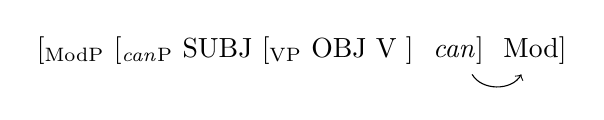
\begin{tikzpicture}[baseline]
		\node[baseline] (A) at (0,0) {[\textsubscript{ModP} [\textsubscript{\emph{can}P} SUBJ [\textsubscript{VP} OBJ V ]};
		\node[right] (can) at (A.east) {\emph{can}]};
	%	\node[right] (B) at (can.east) {]};
		\node[right] (Mod) at (can.east) {Mod]};
%		\node[right] (C) at (Mod.east) {]};
		\draw[bend right,bend right=60,->] (can) to (Mod);
	\end{tikzpicture}
\end{exe}


Here, the subject is base-generated as an argument of the potential suffix (indicated as \emph{can}), and the object is selected by the verb. Furthermore, \citet{shimamurawurmbrand2014} suggest that the potential suffix moves to the Mod(al) head for modal force. I assume (i) that the potential suffix cannot assign the accusative case to the object and (ii) the nominative object and the nominative subject are case-licensed by Tense via Multiple Agree (see \citealt{Ura1999, hiraiwa2001,hiraiwa2005,takahashi2011}); I set aside the movement of the nominative phrases for the moment.\footnote{I assume that nominative case is assigned via (downward) Agree (\citealt{Chomsky2000}). However, see \citet{shimamurawurmbrand2014} for an analysis based on Reverse Agree (see \citealt{Wurmbrand2014} for Reverse Agree). The choice does not affect the discussion in this section.}

\begin{exe}
\ex \label{takaha14} 
	\begin{tikzpicture}[baseline]
		\node[baseline] (A) at (0,0) {[\textsubscript{TP} [\textsubscript{ModP} [\textsubscript{\emph{can}P}};
		\node[right] (subj) at (A.east) {SUBJ\textsubscript{NOM}};
		\node[right] (B) at (subj.east) {[\textsubscript{VP}};
		\node[right] (obj) at (B.east) {OBJ\textsubscript{NOM}};
		\node[right] (C) at (obj.east) {V]};
		\node[right] (can) at (C.east) {\emph{can}]};
%		\node[right] (D) at (can.east) {]};
		\node[right] (Mod) at (can.east) {Mod]};
%		\node[right] (E) at (Mod.east) {]};
		\node[right] (T) at (Mod.east) {T]};
%		\node[right] (F) at (T.east) {]};
		\draw[bend right,bend right=60,->] (can) to (Mod);
		\draw[->] (T) -- ($ (T) - (0,0.6) $) -- ($ (obj) - (0,0.6) $) -- (obj);
		\draw[->] ($ (obj) - (0,0.6) $) -- ($ (subj) - (0,0.6) $) -- (subj);
	\end{tikzpicture}
\end{exe}

\subsection{Putting all the pieces together}
Let us now consider how the above assumptions work together. The contrast that must be accounted for is given below:
\begin{exe}
\ex \label{takaha15}
\begin{xlist}
\ex \label{takaha15a}
\gll {Kodomo-tati-ga} {kanzirensyuu-dake-ga} {tuzuke-rare-ru.}\\
	child-\textsc{pl}-\textsc{nom}  kanji.practice-only-\textsc{nom} continue-can-\textsc{prs}\\
\glt `Children can continue only kanji practice.’ (= (\ref{takaha6a}))\\ 
	`Children can continue kanji practice without doing	any other things.’ (can \textgreater{} only)\\
	‘It is only kanji practice that children can continue.’ (only \textgreater{} can)
\ex \label{takaha15b}
\gll {Kodomo-tati-de} {kanzirensyuu-dake-ga} {tuzuke-rare-ru.}\\
	child-\textsc{pl}-with       kanji.practice-only\textsc{nom} continue-can-\textsc{prs}\\
\glt ‘Children can continue only kanji practice.’ (= (\ref{takaha6b})) \\
‘Children can continue kanji practice without doing any	other things.’ (can \textgreater{} only)\\
‘It is only kanji practice that children can continue.’ (?*only \textgreater{} can)
\end{xlist}
\end{exe}

While the nominative object can take scope over the potential suffix in the presence of the nominative subject, as in (\ref{takaha15a}), the nominative object fails to take scope over the potential suffix in the presence of the instrumental subject, as in (\ref{takaha15b}). Given that the nominative subject moves to TP Spec (see (\ref{takaha12a})), I propose that the nominative object can move above the potential suffix in the presence of the nominative subject (see \citealt{ Koizumi1998, nomura2005}). (\ref{takaha15a}) is thus analyzed as follows:

\begin{exe}
\ex \label{takaha16} 
\begin{forest}
[TP
	[SUBJ\textsubscript{NOM}$_i$]
	[TP
		[OBJ\textsubscript{NOM}$_j$]
		[T'
			[ModP
				[\emph{can}P
					[$t_{i}$]
					[\emph{can'}
						[VP
							[$t_{j}$]
							[V]
						]
						[\emph{can},name=can]
					]
				]
				[Mod,name=mod]
			]
			[T]
		]
	]
]
\draw[->] (can) to[out=south east,in=south east] (mod);
\end{forest}
\end{exe}

The nominative subject is base-generated in \emph{can}P Spec and moves to TP Spec. The nominative object also moves to TP Spec and takes scope over the potential suffix as the nominative object  c-commands the potential suffix after movement. Furthermore, the object can take scope under the potential suffix via reconstruction.\footnote{It might be the case that the nominative object stays within the VP for narrow scope interpretation (see \citealt{nomura2005}; \citealt{ochisaruwatari2014a}).}

Let us now consider the case in which the nominative object co-occurs with the instrumental subject (\ref{takaha15b}). Given that the instrumental subject in transitive sentences stays within \emph{v}P (\ref{takaha12b}), I propose that the instrumental subject in the potential construction stays within \emph{can}P. This entails that the nominative object in (\ref{takaha15b}), which follows the nominative subject, stays within the VP:

\begin{exe}
\ex \label{takaha17}
\begin{forest}
	[TP
		[ModP
			[\emph{can}P
				[SUBJ\textsubscript{INST}]
				[\emph{can'}
					[VP
						[OBJ\textsubscript{NOM}]
						[V]
					]
					[\emph{can}, name=can2]
				]
			]
			[Mod,name=mod2]
		]
		[T]
	]
\draw[->] (can2) to[out=south east,in=south east] (mod2);
\end{forest}
\end{exe}

Given that the instrumental subject stays within the \emph{can}P, the nominative object, which is clearly located below the subject, stays within the VP in (\ref{takaha17}). I assume that quantified elements, including NPs with the focus particle \emph{dake} ‘only’, can take scope without movement into a node of type <t> (see \citealt{Blok2017} for discussion). Thus, the nominative object can be interpreted in its base-generated position.\footnote{Note that the nominative object is not forced to stay within the VP complement in the presence of an instrumental subject; rather, the nominative object can be positioned above the instrumental subject via “overt movement,” in which case the former can take scope over the potential suffix: 
\begin{exe}
\ex 
\begin{xlist}
\ex \label{takahaiaa}
\gll [$_{\textnormal{canP}}$ {Kodomo-tati-de} [$_{\textnormal{VP}}$ {kanzirensyuu-dake-ga} {tuzuke}]-{rare}]-{ru}.\\
{} child-\textsc{pl}-with {} kanji.practice-only-\textsc{nom} continue-can-\textsc{prs}\\
\glt ‘Children can continue only kanji practice.’\\
‘Children can continue kanji practice without doing other things.’ (can \textgreater{} only)\\
‘It is only kanji practice that children can continue.’ (?*only \textgreater{} can) (= (\ref{takaha15b}))

\ex \label{takahaibb}
\gll [$_{\textnormal{TP}}$ {Kanzirensyuu-dake$_{\textnormal{i}}$-ga} [$_{\textnormal{canP}}$ {kodomo-tati-de} [$_{\textnormal{VP}}$ {\textit{t}$_{\textnormal{i}}$} {tuzuke}]-{rare}]-{ru}].\\
{} kanji.practice-only-\textsc{nom} {} child-\textsc{pl}-with {} {} continue-can-\textsc{prs}\\
\glt ‘Children can continue only kanji practice.’\\
‘Children can continue kanji practice without doing other things.’ (can \textgreater{} only)\\
‘It is only kanji practice that children can continue.’ (only \textgreater{} can)
\end{xlist}
\end{exe}
In (\ref{takahaibb}), the nominative object is moved to the sentence-initial position, which I assume to be TP. The nominative object in this example can take scope over the potential suffix. Given that Japanese has scrambling (\citealt{Saito1985}), the movement in question may be scrambling. Alternatively, given that Tense assigns case to the nominative object, the nominative object may undergo raising to TP Spec. I leave the choice open here.}

In sum, I have argued in this section that the obligatory narrow scope interpretation of the nominative object in the presence of the instrumental subject (see (\ref{takaha15b})) follows if we assume that the nominative object in question must stay within \emph{can}P when the former follows the instrumental subject. Note that the above analysis crucially relies on the phrasal complementation approach to restructuring, which posits a full VP structure below a restructuring predicate (i.e., a potential suffix) and requires the nominative object to be base-generated below the potential suffix. The next section discusses an alternative analysis in terms of the complex head approach and shows that such an analysis fails to capture the contrast between (\ref{takaha15a}) and (\ref{takaha15b}).

\section{An alternative: Complex head analysis} \label{takahas4}
This section explores a major alternative analysis of restructuring phenomena in terms of the complex head approach and how the analysis fares with the observations made in this chapter.
In the complex head approach proposed by \citet{SaitoHoshi1998}, the potential suffix and the embedded predicate form a single complex head when the embedded object receives nominative case, which is assumed to be assigned by the potential suffix (\citealt{kuno1973}). In this analysis, all arguments (and adjuncts) that are associated with the embedded predicate are base-generated above the complex head. The analysis thus assigns an identical structure to the nominative object construction with the nominative subject (see (\ref{takaha15a})) and that with the instrumental subject (see (\ref{takaha15b})):

\begin{exe}
\ex \label{takaha18}
	\begin{xlist}
	\ex \label{takaha18a}
		Structure of (\ref{takaha15a}) in complex head analysis:\\
		\begin{forest}
			[VP[SUBJ\textsubscript{NOM}][V'[OBJ\textsubscript{NOM}][V\textsubscript{1can}[V\textsubscript{2}][V\textsubscript{1can}]]]]
		\end{forest} \newpage
	\ex \label{takaha18b}
		Structure of (\ref{takaha15b}) in complex head analysis:\\
		\begin{forest}
			[VP[SUBJ\textsubscript{instr}][V'[OBJ\textsubscript{NOM}][V\textsubscript{1can}[V\textsubscript{2}][V\textsubscript{1can}]]]]]
		\end{forest}
	\end{xlist}
\end{exe}

(\ref{takaha18a}) and (\ref{takaha18b}) verify that the structure of the nominative object construction is the same regardless of the case of the subject: the nominative object is always base-generated above the potential suffix. (\ref{takaha18a}) and (\ref{takaha18b}) thus predict that the scope property of the nominative object should not be affected by the case of the subject. \citet{SaitoHoshi1998} assume (i) that the scope of the potential suffix is determined by the lower segment of the [V1, V1] and (ii) that the potential suffix as a whole (i.e., [V1, V1]) dominates the lower segment of the potential suffix (i.e., V1). The nominative object thus asymmetrically c-commands the lower segment of the potential suffix. The analysis therefore predicts that the nominative object in (\ref{takaha18a}) and (\ref{takaha18b}) should always take scope over the potential suffix. Consequently, it would be difficult to capture the reason the scope of the nominative object depends on the case of the subject.\footnote{The contrast between (\ref{takaha15a}) and (\ref{takaha15b}) also raises a question regarding an approach that posits the covert movement of a quantifier for the wide scope interpretation of the nominative object (see \citealt{bobaljikwurmbrand2007}; \citealt{takahashi2011}; \citealt{FunakoshiTakahashi2014}). Note that \citet{Blok2017} claims that while type mismatch is resolved via type shifting, scope shifting is yielded by quantifier raising. We would then expect that the nominative object (or the focus particle \emph{dake} ‘only’) could covertly move to a position above the potential suffix (I thank one reviewer for pointing this out). Given the unambiguity of (\ref{takaha15b}), we might have to conclude that the relevant covert scope shifting operations are indeed absent in Japanese, in which case we are led to reconsider some observations that are understood in terms of covert scope shifting operations in Japanese (see \citealt{takahashi2011}; \citealt{BobaljikWurmbrand2012}; \citealt{Oku2018}).}

\section{Further considerations}\label{takahas5}
This section considers some consequences of the analysis developed in Section \ref{takahas3}. First, further examinations of relevant examples lead us to one important interpretive property of the potential suffix. The structure of the nominative object construction with the nominative subject (see (\ref{takaha16})) and with the instrumental subject (see (\ref{takaha17})) is given below: 	

\begin{multicols}{2}
\begin{exe}
\ex \label{takaha19}
	\begin{xlist}
	\ex \label{takaha19a} Nominative subject \\(see (\ref{takaha16}))\\
		\begin{forest}
			[TP
				[SUBJ\textsubscript{\textsc{nom}}$_i$]
				[TP
					[OBJ\textsubscript{\textsc{nom}}$_j$]
					[T'
						[ModP
							[\emph{can}P
								[$t_i$]
								[\emph{can'}
									[VP
										[$t_j$]
										[V]
									]
									[\emph{can},name=can3]
								]
							]
							[Mod,name=mod3]
						]
						[T]
					]
				]
			]
			\draw[->] (can3) to[out=south east,in=south east] (mod3);
		\end{forest}
	\ex\label{takaha19b}
		Instrumental subject \\(see (\ref{takaha17})) \\
		\begin{forest}
			[TP[ModP[\emph{can}P[SUBJ\textsubscript{\textsc{inst}}][\emph{can'}[VP[OBJ\textsubscript{\textsc{nom}}][V]][\emph{can},name=can4]]][Mod,name=mod4]][T]]
			\draw[->] (can4) to[out=south east,in=south east] (mod4);
		\end{forest}
	\end{xlist}
\end{exe}
\end{multicols}

The nominative subject in (\ref{takaha19a}) c-commands the potential suffix after the subject movement and is c-commanded by the potential suffix before the subject movement. The instrumental subject in (\ref{takaha19b}) c-commands the potential suffix before movement of the latter and is c-commanded by the raised potential suffix. Therefore, it may be predicted that the nominative and instrumental subjects can take scope over or under the potential suffix. However, the following examples show that both types of subject interact with the potential suffix unambiguously:

\begin{exe}
\ex \label{takaha20}
\begin{xlist}
\ex \label{takaha20a}
	\gll {Kodomo-tati}-{dake-ga} {kanzirensyuu-ga} {tuzuke-rare-ru.}\\
	child-\textsc{pl}-only-\textsc{nom}  kanji.practice-\textsc{nom} continue-can-\textsc{prs}\\\\
	\glt `Only children can continue kanji practice.’\\ 
	`Children can continue kanji practice without other people around.’ (*can \textgreater{} only)\\
	‘It is only children who can continue kanji practice.’ (only \textgreater{} not)
	
\ex \label{takaha20b}
	\gll {Kodomo-tati}-{dake-de} {kanzirensyuu-ga} {tuzuke-rare-ru.}\\
	child-\textsc{pl}-only-with       kanji.practice-\textsc{nom} continue-can-\textsc{prs}\\
	\glt ‘Children can continue only kanji practice.’ (= (\ref{takaha6b})) \\
	`Only children can continue kanji practice.’\\ 
	`Children can continue kanji practice without other people around.’ (can \textgreater{} only)\\
	‘It is only children who can continue kanji practice.’ (*only \textgreater{} not)
\end{xlist}
\end{exe}

While the nominative subject in (\ref{takaha20a}) necessarily takes scope over the potential suffix, the instrumental subject in (\ref{takaha20b}) takes scope under the potential suffix. I assume that the obligatory wide scope interpretation of the nominative subject in (\ref{takaha20a}) reduces to a well-known observation in the literature that sentence-initial nominative phrases must receive exhaustive-listing interpretation when a predicate is individual-level (see \citealt{kuno1973}). The obligatory narrow scope interpretation of the instrumental subject in (\ref{takaha20b}) follows if the potential suffix is interpreted only in its derived position, which asymmetrically c-commands the instrumental subject. \footnote{Note that the contrast between (\ref{takaha20a}) and (\ref{takaha20b}) provides another argument against complex head analysis; as such analysis requires that the subjects always be base-generated above the potential suffix, it fails to capture the availability of the narrow scope interpretation of the instrumental subject observed in (\ref{takaha20b}).}

Furthermore, the proposed analysis predicts that the nominative object can take scope over the potential suffix when a non-nominative subject moves to TP Spec. This is because when the subject moves into TP Spec, the object that follows the subject can also move into TP Spec. This is illustrated below:

\begin{exe}
\ex \label{takaha21}
	\begin{xlist}
	\ex \label{takaha21a} 
		\begin{tikzpicture}[baseline]
			\node[baseline] (A) at (0,0) {[\textsubscript{\textsc{tp}}};
			\node[right] (landing) at (A.east) {}; 
			\node[right] (C) at (landing.east) {[\textsubscript{\textsc{ModP}} [\textsubscript{\emph{can}P} SUBJ [\textsubscript{\textsc{vp}}};
			\node[right] (obj) at (C.east) {OBJ\textsubscript{\textsc{nom}}};
			\node[right] (D) at (obj.east) {V] \emph{can}] Mod] T]};
			\draw[->] (obj) -- ($ (obj) - (0,0.5) $) to node {*} ($ (landing) - (0,0.5) $) --  (landing);	
		\end{tikzpicture}
	\ex \label{takaha21b}
		\begin{tikzpicture}[baseline]
			\node[baseline] (A) at (0,0) {[\textsubscript{\textsc{tp}} SUBJ$_{\textnormal{i}}$};
			\node[right] (obj) at (A.east) {OBJ\textsubscript{\textsc{nom}}$_{\textnormal{j}}$};
			\node[right] (B) at (obj.east) {[\textsubscript{\textsc{ModP}} [\textsubscript{\emph{can}P} $t_{\textnormal{i}}$ [\textsubscript{\textsc{vp}}};
			\node[right] (trace) at (B.east) {$t_\textnormal{i}$};
			\node[right] (C) at (trace.east) {V] \emph{can}] Mod] T]};
			\draw[->] (trace) -- ($(trace)-(0,0.5)$) -- ($(obj)-(0,0.5)$) -- (obj);
		\end{tikzpicture}
	\end{xlist}
\end{exe}

When the subject stays within canP Spec, the nominative object following the subject must stay within the VP. This is the case of the nominative object with the instrumental subject (see (\ref{takaha21a})). Conversely, when the subject moves into TP Spec, the nominative object can also move into TP Spec. This is the case of the nominative object with the nominative subject (see (\ref{takaha21b})). We then expect that the nominative object can move into TP Spec when a non-nominative subject moves into TP Spec. This prediction is borne out. In contrast to the instrumental subject, the dative subject can take scope over negation:

\begin{exe}
\ex \label{takaha22}
\begin{xlist}
\ex \label{takaha22a}
	\gll {Kodomo-tati}-{dake-de} {kanzirensyuu-ga} {tuzuke-rare-na-i.}\\
	child-\textsc{pl}-only-with  kanji.practice-\textsc{nom} continue-can-\textsc{neg}-\textsc{prs}\\\\
	\glt `Only children can't continue kanji practice.’\\ 
	‘It is not the case that only children can continue kanji practice.’ (not \textgreater{} only)\\
	‘It is only children who cannot continue kanji practice.’ (*only \textgreater{} not)
    	
\ex \label{takaha22b}
	\gll {Kodomo-tati}-{dake-ni} {kanzirensyuu-ga} {tuzuke-rare-na-i.}\\
	child-\textsc{pl}-only-\textsc{dat}       kanji.practice-\textsc{nom} continue-can-\textsc{neg}-\textsc{pst}\\
	\glt ‘Only children cannot continue kanji practice.’\\
	‘It is not the case that only children can continue kanji practice of kanji.’ (?not  \textgreater{} only)\\	           ‘It is only children who cannot continue kanji practice.’ (only \textgreater{} not)
\end{xlist}
\end{exe}

Although the instrumental subject in (\ref{takaha22a}) cannot take scope over negation, the dative subject in (\ref{takaha22b}) can take scope over negation. The contrast indicates that while the instrumental subject stays within \emph{can}P, the dative subject moves into TP Spec, just like the nominative subject (see \citealt{Ura1999}; \citealt{Kishimoto2010}):

\begin{exe}
\ex \label{takaha23}
\begin{xlist}
\ex \label{takaha23a}
	[$_{\textnormal{\textsc{tp}}}$ SUBJ$_{\textnormal{\textsc{nom/dat}}}$ \hspace{1mm} [$_{NegP}$ [$_{\textnormal{\textsc{canP}}}$ \hspace{8mm} \emph{t$_{\text{i}}$} \hspace{8mm}] Neg] T] (see (\ref{takaha12a}))
\ex \label{takaha23b}
	[$_{\textnormal{\textsc{tp}}}$ \hspace{22mm} [$_{NegP}$ [$_{\textnormal{\textsc{canP}}}$ \hspace{1mm} SUBJ$_{\textnormal{\textsc{inst}}}$ \hspace{2.6mm}] Neg] T] (see (\ref{takaha12b}))
\end{xlist}
\end{exe}

We would then expect that the nominative object that co-occurs with the dative subject can take scope over the potential suffix. This prediction is borne out (see \citealt{Ura1999, takahashi2011}):

\begin{exe}
\ex \label{takaha24}
\begin{xlist}
\ex \label{takaha24a}
	\gll {Kodomo-tati-de} {kanzirensyuu-dake-ga} {tuzuke-rare-ru.}\\
	child-\textsc{pl}-with  kanji.practice-only-\textsc{nom} continue-can-\textsc{prs}\\\\
	\glt ‘Children can continue only kanji practice.’ (= (\ref{takaha15b}))\\ 
	‘Children can continue kanji practice without doing any other things.’ (can \textgreater{} only)\\
	‘It is only kanji practice that children can continue.’ (?*only \textgreater{} can)
    	
\ex \label{takaha24b}
	\gll {Kodomo-tati-ni} {kanzirensyuu-dake-ga} {tuzuke-rare-ru.}\\
	child-\textsc{pl}-\textsc{dat}       kanji.practice-only-\textsc{nom} continue-can-\textsc{prs}\\
	\glt ‘Children can continue only kanji practice.’ \\
	‘Children can continue kanji practice without doing any other things.’ (can \textgreater{} only)\\
	‘It is only kanji practice that children can continue.’ (only \textgreater{} can)
\end{xlist}
\end{exe}

As we have observed above, the nominative object in (\ref{takaha24a}), which co-occurs with the instrumental subject, only takes scope under the potential suffix. By contrast, the nominative object in (\ref{takaha24b}), which co-occurs with the dative subject, can take scope over the potential suffix. The contrast between (\ref{takaha24a}) and (\ref{takaha24b}) provides further credence to the current analysis, which dictates that the nominative object can take scope over the potential suffix when the string-vacuous movement of the latter is not blocked by the intervening subject.

In sum, I have discussed some consequences of the analysis developed in the previous sections. In particular, I have shown (i) that the scope of the potential suffix is determined in its derived position and (ii) that nominative objects that co-occur with a non-nominative subject sometimes take scope over the potential suffix.

\section{Conclusion}\label{takahas6}
In this chapter, I have provided a new argument for the phrasal complementation approach to restructuring on the basis of some new observations concerning the scope properties of nominative objects in the Japanese potential construction. Specifically, I have shown that the nominative object must take scope under the potential suffix in the presence of the instrumental subject, which the phrasal complementation approach accommodates. In contrast, the observation in question is hard to account for with the complex head approach, which always requires the nominative object to be base-generated above the potential suffix. I have also shown that the wide scope behavior of the nominative object interacts with subject movement on the basis of the analysis of the nominative object that co-occurs with the dative subject.



\begin{comment}
\newpage
\section*{Abbreviations}
\begin{tabularx}{.45\textwidth}{lQ}
... & \\
... & \\
\end{tabularx}
\begin{tabularx}{.45\textwidth}{lQ}
... & \\
... & \\
\end{tabularx}
\end{comment}

\section*{Acknowledgements}
It is my pleasure to dedicate this chapter to Susi Wurmbrand, who is an extremely committed and inspiring teacher. I would like to thank her for many hours of discussion at the University of Connecticut; these discussions served as a basis of my dissertation (\citealt{takahashi2011}) and my subsequent research. I would also like to thank her for producing many stimulating works on infinitives and many other topics, from which I have learned a lot. I am also grateful to Sato Ebina, Hisako Takahashi, Naoto Tomizawa, and two reviewers for helpful comments and/or discussions. The research reported herein was supported in part by JSPS KAKENHI Grant Number 20K00535. I am solely responsible for any errors in the text.



\sloppy \printbibliography[heading=subbibliography,notkeyword=this]

\end{document}
